\chapter{Views}

% What is a view? Referere til kapittel 9

Different views support different goals and uses.
The views you should document depend on the uses you expect to make of the documentation.

% Relevant views

% Fremgangsmåte
% 1. Produce a candidate view list
% 2. Combine views
% 3. Prioritize

As described in chapter \ref{cha:architectural_viewpoint}, the views deemed the most useful for the development of LaHAW is the \emph{logic}, \emph{development} and \emph{process} views from the 4+1 view model.
 






\section{Logic view}

% 1. Primariy presentation
% 2. Element catalog
% 3. Context diagram
% 4. Variability
% 5. Architecture background
% 6. Glossary of terms
% 7. Other information

\begin{figure}[ht]
    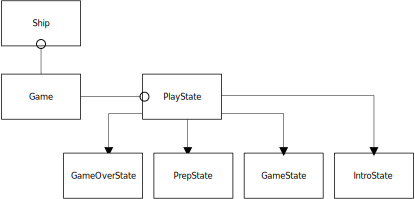
\includegraphics[width=\textwidth]{LogicalView.png}
    \caption{UML Class diagram illustrating the Logical View}
    \label{fig:LogicalView}
\end{figure}

Figure \ref{fig:LogicalView} shows a simplified overview of the different classes, usages and object inheritances. Notation is based on the Logical View notation by Kructhen\cite{kruchten}. This decomposition helps identify elements that are shared across the system.

\texttt{GameOverState}, \texttt{PrepState}, \texttt{GameState} and \texttt{IntroState} all extend a common \texttt{PlayState} class, and describes the different states the game can exist in at a given time.

The main \texttt{Game} class functions as the game's main controller, and controls the state stack. The \texttt{Ship} object instantiates the different ship types with a given set of attributes, which in turn is controlled by the main \texttt{Game} class.

Other states and objects are discussed earlier in this report, but are not represented in this diagram. The main reason for this descision is to keep the diagram simple and easy to read, and that the ignored features are either redundant or too specific.



\section{Development view}


\begin{figure}[ht]
    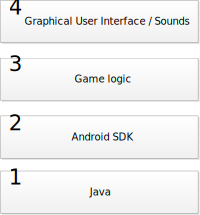
\includegraphics{DevelopmentView.png}
    \caption{Development View Architecture Layer Diagram}
    \label{fig:DevelopmentView}
\end{figure}

Figure \ref{fig:DevelopmentView} illustrates 


% Foreslår å sløyfe Java.
At the very bottom you find the Java layer. This is 


Below this, the game logic layer. This layer deals with the internal game states and logic that drives the game. This information is derived from the Android SDK layer below, and communicated to the GUI layer above.


At the top the graphical user interface and sound assets are contained. As mentioned above, this derives its information from the layer below.

If implemented properly, this will make it possible to completely replace one or more of the layers to port or maintain the code.


This will aid the maintainability, as separating the different parts of the code base into layers will make it possible to change and maintain and not break code in different layers.

Additionally, this will aid the portability of the game. If the game is to be ported to Apple iOS, we can replace the lowermost layers, keeping the uppermost GUI and sound layer, adapting the game logic code to use the new API.




% Software packaged in small chunks: 
% – Subsystems can be developed by one or few developers. 
% – Subsystems are organized in hierarchy of layers. 
% – Each layer provides well-defined interface to layers above.


\section{Process view}
Non-functional requirements - performance, availability
    
\begin{figure}[ht]
    \includegraphics[angle=90, scale=0.8]{ProcessLayer.png}
    \caption{Process View Activity Diagram}
    \label{fig:ActivityDiagram}
\end{figure}

Figure \ref{fig:ActivityDiagram} shows …

When a player wants to start a game, the player will be be presented with the game's main menu. From here, the player will be able to choose \emph{Start game}, where, after placing its boats, the game will enter the main \emph{Game State}.

After both of the players are ready, t

The player will now have go at hitting the opponent's warships.


Note that this diagram is a simplified version, and does not show the user customisation part\footnote{E.g. selection of player colour and setting a player name.} of the application. This would have been available from the \emph{Main Menu} activity.




\section{Scenario view}



\section{Physical view}
Reliability, Scalability